\section{Hiệu năng thuật toán}
\label{sec:performance}
Trong phần này chúng ta sẽ xem xét hiệu năng của ALNS. Để thấy rõ sự khác biệt, các đồ thị được trình bày dưới đây là kết quả cho cấu hình với số lượng yêu cầu rất lớn ($1000$ yêu cầu) và số lượng yêu cầu trung bình ($400$ yêu cầu). Ngoài ra, để tránh dài dòng, các đồ thị được thể hiện cho 3 cầu hình C1\_x\_1, R1\_x\_1, RC1\_x\_1 ($x = 10$ cho tập $1000$ yêu cầu, và $x=4$ cho tập $400$ yêu cầu). Hiệu năng của các thuật toán đối với các cấu hình khác là tương tự. Chúng ta sẽ so sánh hiệu năng của ALNS nguyên bản, B-ALNS và một framework rất nổi tiếng trong cộng đồng là \code{Google OR-Tools}. Hiệu năng được so sánh cho cả phiên bản đơn luồng và đa luồng của ALNS \footnote[1]{Các giá trị hàm mục tiêu hay số xe được biểu diễn theo thời gian chạy của thuật toán. Một số đường "dừng sớm" trước thời giam timeout nghĩa là từ đó đến hết thời gian timeout thuật toán chưa tìm thêm được nghiệm tốt hơn.}.

\subsection{Giá trị hàm mục tiêu}

Trước hết, ta xem xét giá trị hàm mục tiêu theo thời gian. Các đồ thị dưới đây cho thấy giá trị hàm mục tiêu theo thời gian khi chạy thuật toán với thời gian chạy 60 giây và được phóng đại để nhìn rõ hơn sự khác biệt trong 10 giây đầu tiên đối với các cấu hình $1000$ và lần lượt là 10 giây và 1 giây đối với cấu hình $400$ yêu cầu. Đồ thị được chia làm 3 phần tương ứng với 3 lớp cấu hình khác nhau là C, R và RC. Không có thuật toán nào được sừ dụng tốt hơn các thuật toán còn lại ở mọi mặt, chúng đều có sự đánh đổi. Chúng ta sẽ cùng phân tích điểm mạnh và điểm yếu của từng chiến thuật trong các giai đoạn và mục đích khác nhau. Từ đó ta có thể đưa ra gợi ý về việc sử dụng thuật toán nào cho mục đích cụ thể.

\begin{figure}[H] % places figure environment here   
  \label{fig:perf_ct_c1_10}
  \begin{subfigure}{.5\textwidth}
    \centering
    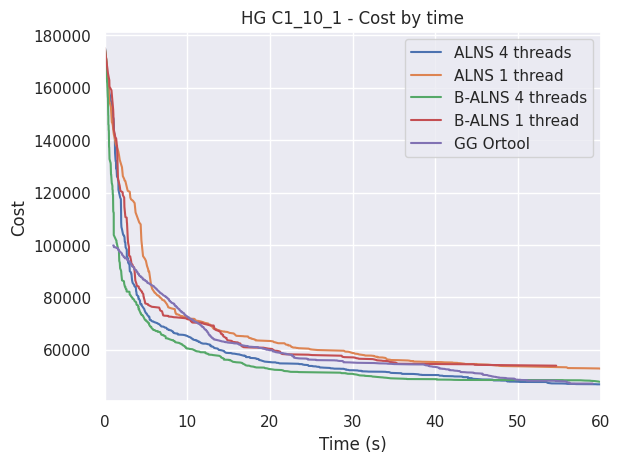
\includegraphics[width=1\linewidth]{figures/cost_time_60s_C1_10_1.png}
    \caption{60s}
    \label{fig:perf_ct_c1_10_60s}
  \end{subfigure}%
  \begin{subfigure}{.5\textwidth}
    \centering
    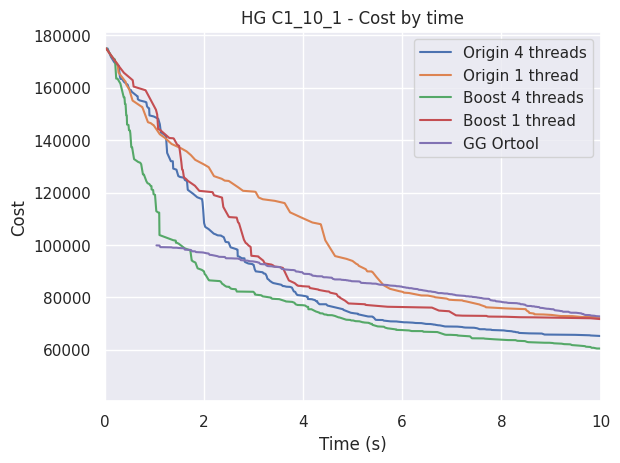
\includegraphics[width=1\linewidth]{figures/cost_time_10s_C1_10_1.png}
    \caption{10s}
    \label{fig:perf_ct_c1_10_10s}
  \end{subfigure}
  \caption{Giá trị hàm mục tiêu theo thời gian, cấu hình C1\_10\_1}
\end{figure}

\begin{figure}[H] % places figure environment here   
  \label{fig:perf_ct_r1_10}
  \begin{subfigure}{.5\textwidth}
    \centering
    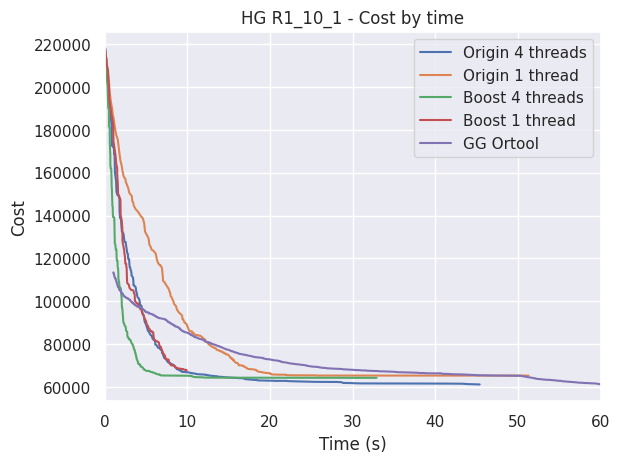
\includegraphics[width=1\linewidth]{figures/cost_time_60s_R1_10_1.png}
    \caption{60s}
    \label{fig:perf_ct_r1_10_60s}
  \end{subfigure}%
  \begin{subfigure}{.5\textwidth}
    \centering
    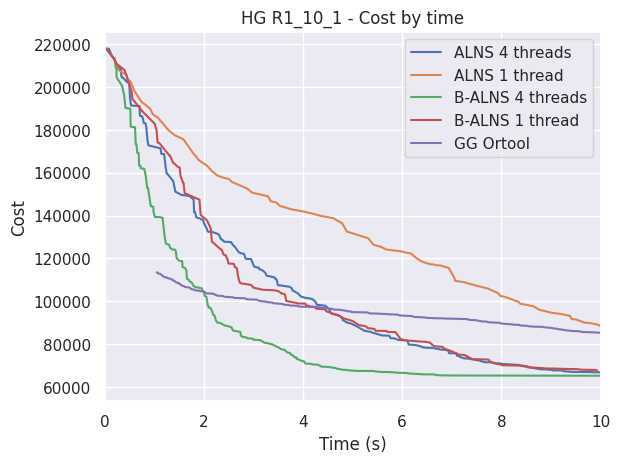
\includegraphics[width=1\linewidth]{figures/cost_time_10s_R1_10_1.png}
    \caption{10s}
    \label{fig:perf_ct_r1_10_10s}
  \end{subfigure}
  \caption{Giá trị hàm mục tiêu theo thời gian, cấu hình R1\_10\_1}
\end{figure}

\begin{figure}[H] % places figure environment here   
  \label{fig:perf_ct_rc1_10}
  \begin{subfigure}{.5\textwidth}
    \centering
    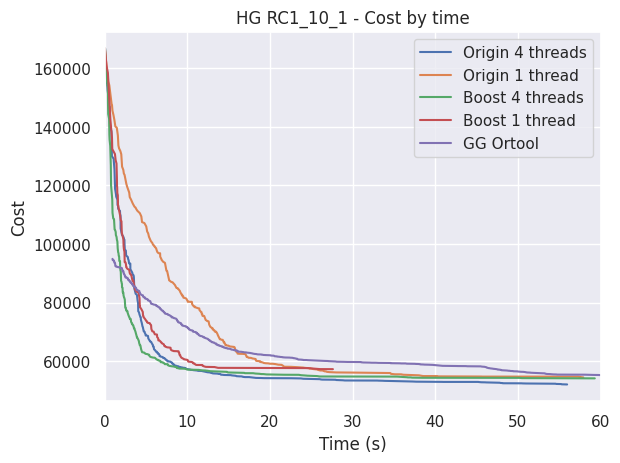
\includegraphics[width=1\linewidth]{figures/cost_time_60s_RC1_10_1.png}
    \caption{60s}
    \label{fig:perf_ct_rc1_10_60s}
  \end{subfigure}%
  \begin{subfigure}{.5\textwidth}
    \centering
    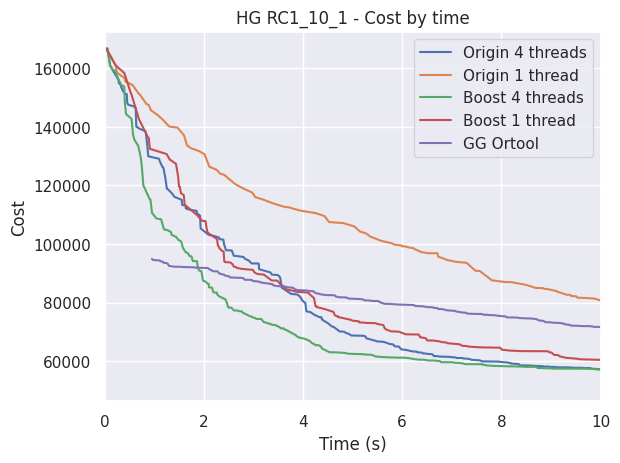
\includegraphics[width=1\linewidth]{figures/cost_time_10s_RC1_10_1.png}
    \caption{10s}
    \label{fig:perf_ct_rc1_10_10s}
  \end{subfigure}
  \caption{Giá trị hàm mục tiêu theo thời gian, cấu hình RC1\_10\_1}
\end{figure}

\begin{figure}[H] % places figure environment here   
  \label{fig:perf_ct_c1_4}
  \begin{subfigure}{.5\textwidth}
    \centering
    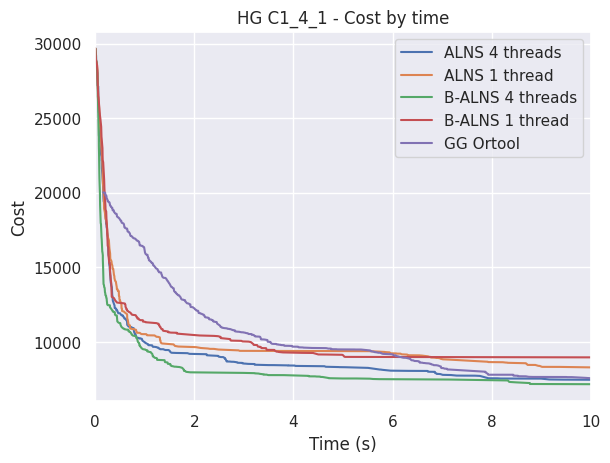
\includegraphics[width=1\linewidth]{figures/cost_time_10s_C1_4_1.png}
    \caption{10s}
    \label{fig:perf_ct_c1_4_10s}
  \end{subfigure}%
  \begin{subfigure}{.5\textwidth}
    \centering
    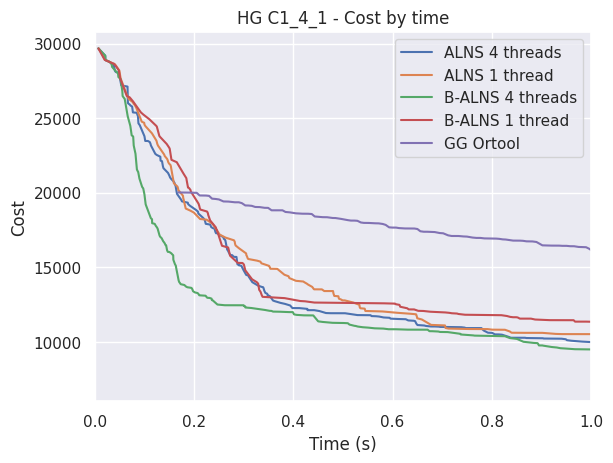
\includegraphics[width=1\linewidth]{figures/cost_time_1s_C1_4_1.png}
    \caption{1s}
    \label{fig:perf_ct_c1_4_1s}
  \end{subfigure}
  \caption{Giá trị hàm mục tiêu theo thời gian, cấu hình C1\_4\_1}
\end{figure}

\begin{figure}[H] % places figure environment here   
  \label{fig:perf_ct_r1}
  \begin{subfigure}{.5\textwidth}
    \centering
    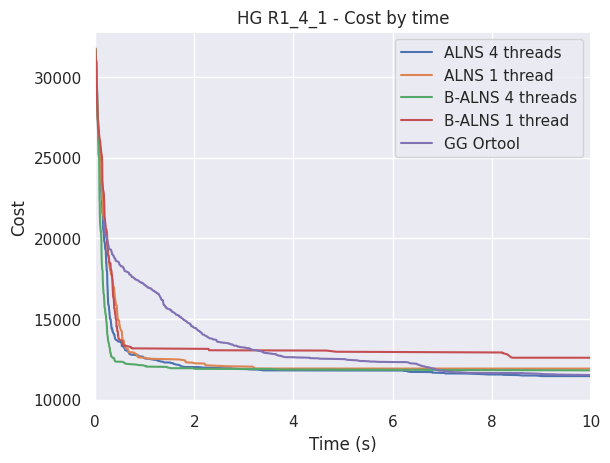
\includegraphics[width=1\linewidth]{figures/cost_time_10s_R1_4_1.png}
    \caption{10s}
    \label{fig:perf_ct_r1_60s}
  \end{subfigure}%
  \begin{subfigure}{.5\textwidth}
    \centering
    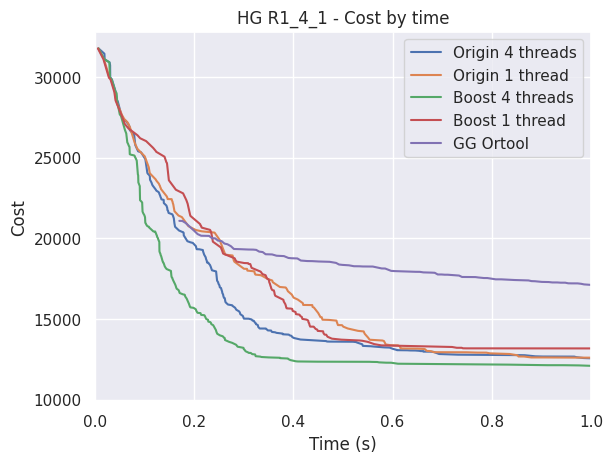
\includegraphics[width=1\linewidth]{figures/cost_time_1s_R1_4_1.png}
    \caption{1s}
    \label{fig:perf_ct_r1_10s}
  \end{subfigure}
  \caption{Giá trị hàm mục tiêu theo thời gian, cấu hình R1\_4\_1}
\end{figure}

\begin{figure}[H] % places figure environment here   
  \label{fig:perf_ct_rc1_4}
  \begin{subfigure}{.5\textwidth}
    \centering
    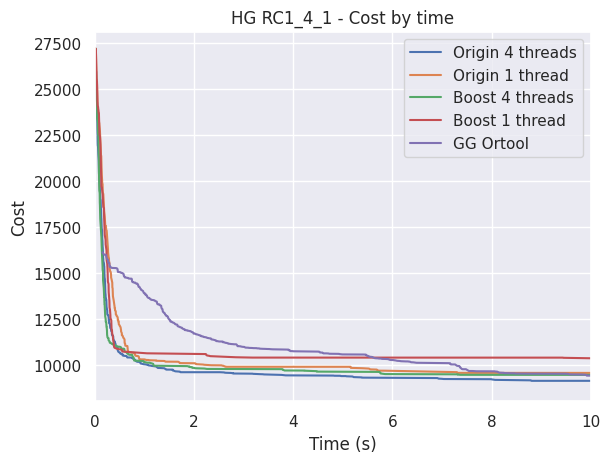
\includegraphics[width=1\linewidth]{figures/cost_time_10s_RC1_4_1.png}
    \caption{10s}
    \label{fig:perf_ct_rc1_4_10s}
  \end{subfigure}%
  \begin{subfigure}{.5\textwidth}
    \centering
    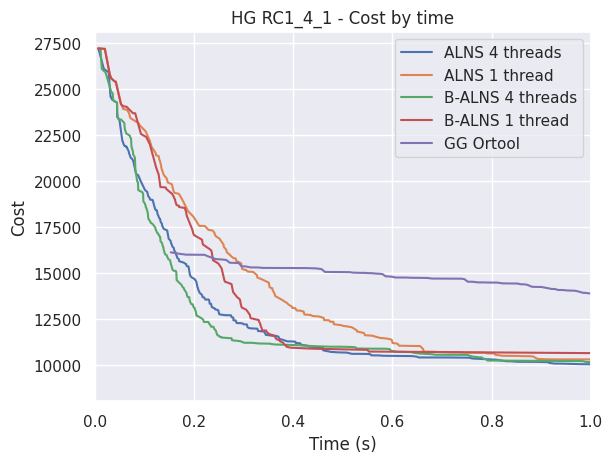
\includegraphics[width=1\linewidth]{figures/cost_time_1s_RC1_4_1.png}
    \caption{1s}
    \label{fig:perf_ct_rc1_4_1s}
  \end{subfigure}
  \caption{Giá trị hàm mục tiêu theo thời gian, cấu hình RC1\_4\_1}
\end{figure}

Với thời gian chạy lâu, các thuật toán đều chững lại bởi khi đó các tuyến đường đã khá chật chội, việc "sửa chữa" là khó khăn hơn giai đoạn đầu rất nhiều. Nói cách khác, thuật toán bị bẫy trong nghiệm tối ưu cục bộ. Khi chạy thuật toán với thời gian lâu hơn (timeout mười phút), tác giả nhận thấy hàm mục tiêu không giảm đáng kể nữa. Chính vì thế, thời gian chạy 60 giây được lựa chọn để vừa phù hợp với thực tế và tránh việc chạy quá lâu.

Ta thấy một xu hướng rõ ràng, trong giai đoạn đầu, B-ALNS tăng tốc hiệu năng của ALNS một cách đáng kể. Với tập dữ liệu $1000$ yêu cầu, thời gian chạy dưới 10 giây, B-ALNS đơn luồng cho hiệu năng gần như tương đương với ALNS với 4 luồng. Nghĩa là, B-ALNS tiết kiệm khoảng $75\%$ tài nguyên CPU để đạt kết quả tương đương với ALNS trong thời gian chạy dưới 10 giây. Chưa kể, bộ nhớ cũng được tiết kiệm một cách đáng kể khi B-ALNS sử dụng 1 luồng thay vì 4 luồng. Khi so sánh với ALNS đơn luồng, B-ALNS đơn luồng cho hiệu năng vượt trội. Với thời gian chạy dưới 2 giây B-ALNS cho chất lượng nghiệm tốt hơn từ khoảng $20\%$ tới $30\%$ so với ALNS. Đối với tập dữ liệu có số lượng yêu cầu trung bình ($400$ yêu cầu), B-ALNS đơn luồng không có lợi thế so với ALNS đơn luồng, tuy nhiên hiệu năng đa luồng vẫn tốt hơn ALNS. Điều này cho thấy, B-ALNS có thể được sử dụng để giải quyết các bài toán lớn với tài nguyên hạn chế. Với cấu hình $400$ yêu cầu, B-ALNS đa luồng cho hiệu năng bỏ xa ALNS với thời gian chạy dưới $0.2$ giây và luôn tốt hơn trong thời gian chạy dưới $1$ giây.

Khi so sánh với \code{Google OR-Tools}, ta thấy rằng, \code{Google OR-Tools} cho hiệu năng tốt trong thời gian chạy từ 2 đến 4 giây đầy tiên (tập $1000$ yêu cầu). Tuy nhiên với thời gian chạy dưới 1 giây, \code{Google OR-Tools} không thể cho ra kết quả. Với thời gian chạy lâu hơn, \code{Google OR-Tools} cho hiệu năng không tốt bằng ALNS hay B-ALNS. Với cấu hình $400$ yêu cầu, nhìn chung hiệu năng của B-ALNS cũng như ALNS bỏ xa \code{Google OR-Tools}.

Như vậy đối với các nghiệp vụ yêu cầu một kết quả tốt trong thời gian ngắn, B-ALNS là lựa chọn tốt nhất. Khi tiến hành đo đạc với thời gian chạy dài (timeout lớn hơn một phút), tác giả nhận thấy rằng, ALNS là tốt nhất trong các thuật toán được đề cập ở đây. Tuy nhiên chất lượng nghiệm tốt hơn B-ALNS thường không quá $1\%$. Các kết quả được chỉ ra trong phần trước là giá trị hàm mục tiêu khi sử dụng ALNS nguyên bản.

\subsection{Số xe}

Chúng ta cũng nhận thấy một xu hướng tương tự như khi so sánh hiệu năng của các thuật toán khi sử dụng độ đo là giá trị hàm mục tiêu. B-ALNS cho hiệu năng vượt trội trong giai đoạn đầu. B-ALNS đơn luồng cho hiệu năng tương đương với ALNS với 4 luồng. Với cấu hình lớp R ($1000$ yêu cầu), B-ALNS tiết kiệm được khoảng $30\%$ số xe so với ALNS trong thời gian chạy từ 2 tới 4 giây! Tương tự, với cấu hình $400$ yêu cầu, B-ALNS giảm số xe nhanh hơn đáng kể so với ALNS trong thời gian chạy ngắn (dưới $0.2$ giây).  Việc tiết kiệm hàng trăm xe có ý nghĩa rất lớn trong thực tế. Thường thì chi phí cho một xe (thuê, hoặc mua, nhiên liệu, chi phí cho tài xế, ...) là rất lớn. Việc tiết kiệm số xe sẽ giúp giảm chi phí vận hành của doanh nghiệp một cách đáng kể. 

Với thời gian chạy lâu hơn, đương nhiên chúng ta rất khó để giảm được số xe nữa, vì hầu hết các tuyến đường đến lúc này đã chật chội hơn đáng kể so với giai đoạn đầu.

\begin{figure}[H] % places figure environment here   
  \label{fig:perf_ct_c1_10}
  \begin{subfigure}{.5\textwidth}
    \centering
    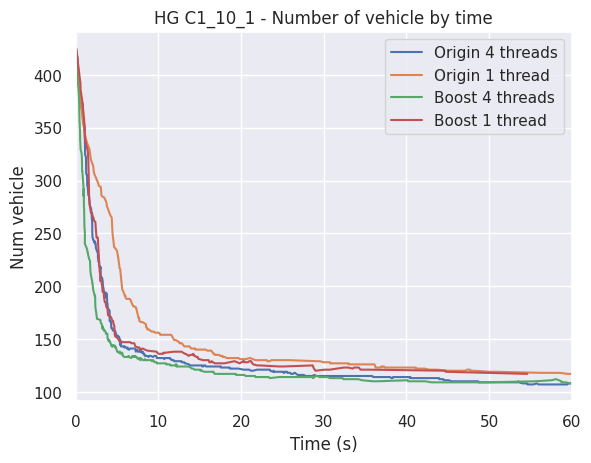
\includegraphics[width=0.9\linewidth]{figures/nv_time_60s_C1_10_1.png}
    \caption{60s}
    \label{fig:perf_ct_c1_10_60s}
  \end{subfigure}%
  \begin{subfigure}{.5\textwidth}
    \centering
    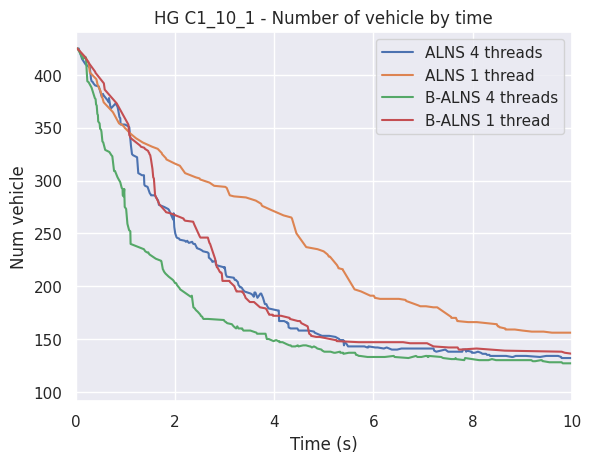
\includegraphics[width=0.9\linewidth]{figures/nv_time_10s_C1_10_1.png}
    \caption{10s}
    \label{fig:perf_ct_c1_10_10s}
  \end{subfigure}
  \caption{Số xe sử dụng theo thời gian, cấu hình C1\_10\_1}
\end{figure}

\begin{figure}[H] % places figure environment here   
  \label{fig:perf_ct_r1_10}
  \begin{subfigure}{.5\textwidth}
    \centering
    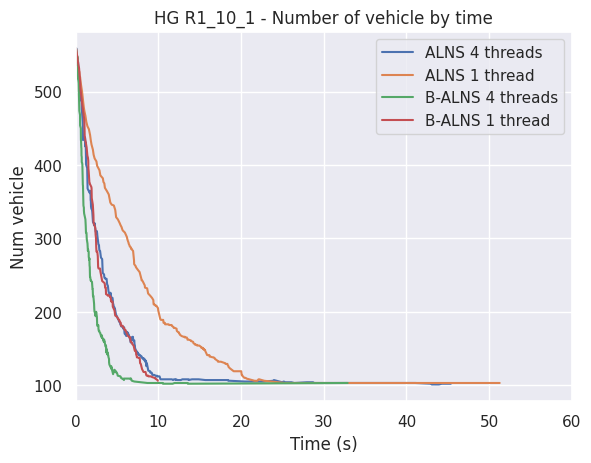
\includegraphics[width=0.9\linewidth]{figures/nv_time_60s_R1_10_1.png}
    \caption{60s}
    \label{fig:perf_ct_r1_10_60s}
  \end{subfigure}%
  \begin{subfigure}{.5\textwidth}
    \centering
    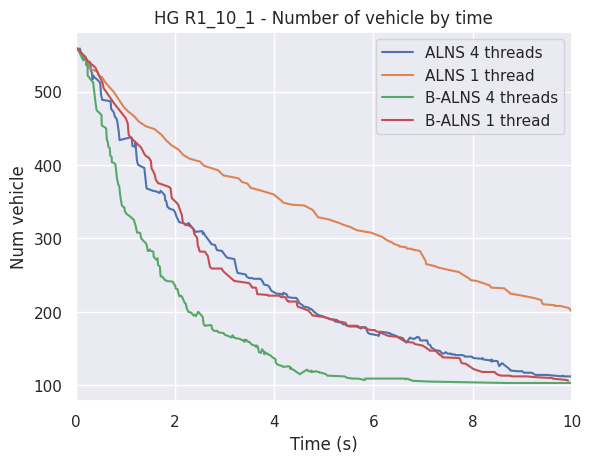
\includegraphics[width=0.9\linewidth]{figures/nv_time_10s_R1_10_1.png}
    \caption{10s}
    \label{fig:perf_ct_r1_10_10s}
  \end{subfigure}
  \caption{Số xe sử dụng theo thời gian, cấu hình R1\_10\_1}
\end{figure}

\begin{figure}[H] % places figure environment here   
  \label{fig:perf_ct_rc1}
  \begin{subfigure}{.5\textwidth}
    \centering
    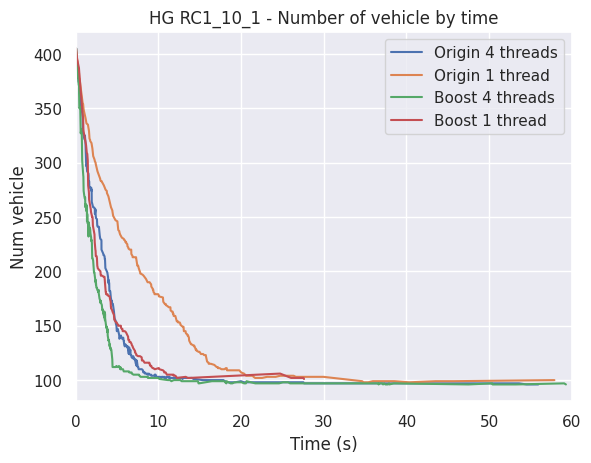
\includegraphics[width=0.9\linewidth]{figures/nv_time_60s_RC1_10_1.png}
    \caption{60s}
    \label{fig:perf_ct_rc1_60s}
  \end{subfigure}%
  \begin{subfigure}{.5\textwidth}
    \centering
    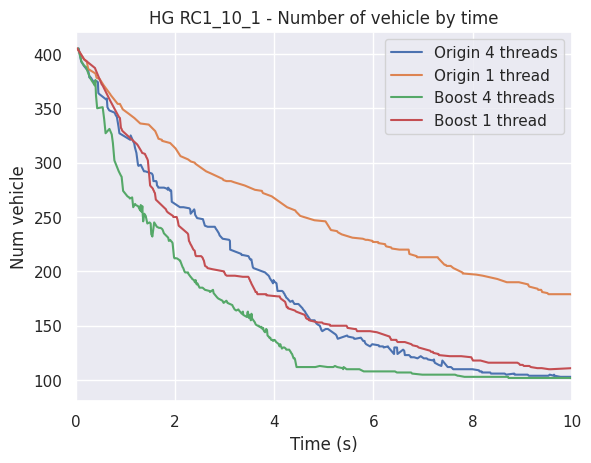
\includegraphics[width=0.9\linewidth]{figures/nv_time_10s_RC1_10_1.png}
    \caption{10s}
    \label{fig:perf_ct_rc1_10s}
  \end{subfigure}
  \caption{Số xe sử dụng theo thời gian, cấu hình RC1\_10\_1}
\end{figure}

\begin{figure}[H] % places figure environment here   
  \label{fig:perf_ct_c1_4}
  \begin{subfigure}{.5\textwidth}
    \centering
    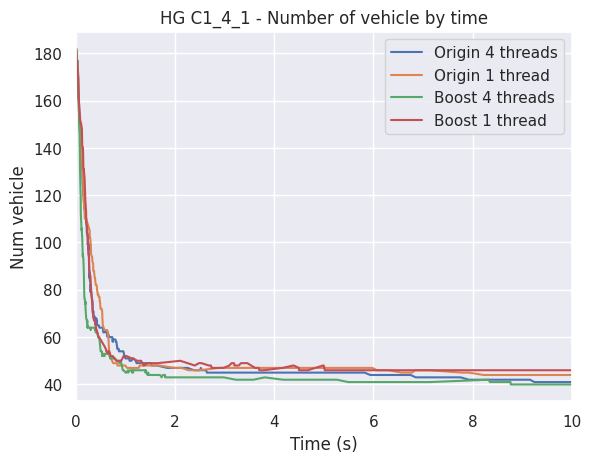
\includegraphics[width=0.9\linewidth]{figures/nv_time_10s_C1_4_1.png}
    \caption{10s}
    \label{fig:perf_ct_c1_4_10s}
  \end{subfigure}%
  \begin{subfigure}{.5\textwidth}
    \centering
    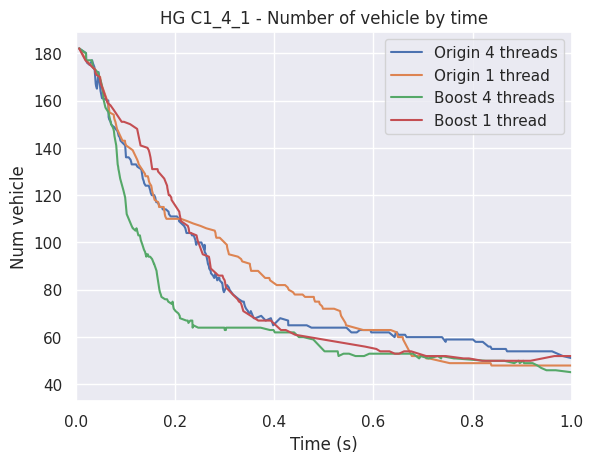
\includegraphics[width=0.9\linewidth]{figures/nv_time_1s_C1_4_1.png}
    \caption{1s}
    \label{fig:perf_ct_c1_4_1s}
  \end{subfigure}
  \caption{Số xe sử dụng theo thời gian, cấu hình C1\_4\_1}
\end{figure}

\begin{figure}[H] % places figure environment here   
  \label{fig:perf_ct_r1_4}
  \begin{subfigure}{.5\textwidth}
    \centering
    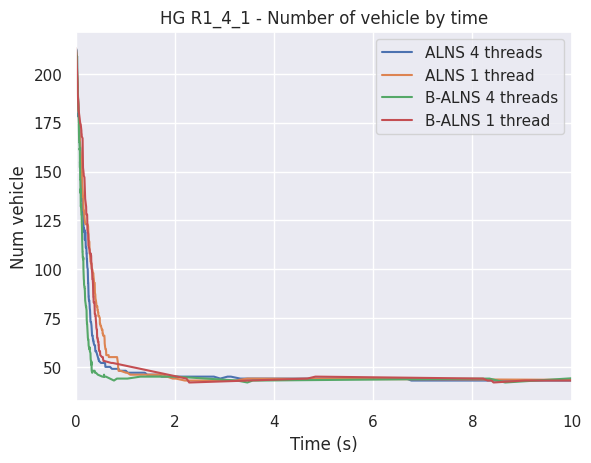
\includegraphics[width=0.9\linewidth]{figures/nv_time_10s_R1_4_1.png}
    \caption{10s}
    \label{fig:perf_ct_r1_4_10s}
  \end{subfigure}%
  \begin{subfigure}{.5\textwidth}
    \centering
    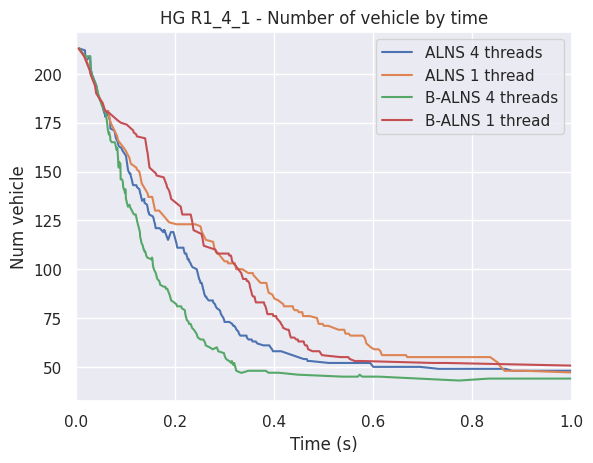
\includegraphics[width=0.9\linewidth]{figures/nv_time_1s_R1_4_1.png}
    \caption{1s}
    \label{fig:perf_ct_r1_4_1s}
  \end{subfigure}
  \caption{Số xe sử dụng theo thời gian, cấu hình R1\_4\_1}
\end{figure}

\begin{figure}[H] % places figure environment here   
  \label{fig:perf_ct_rc1}
  \begin{subfigure}{.5\textwidth}
    \centering
    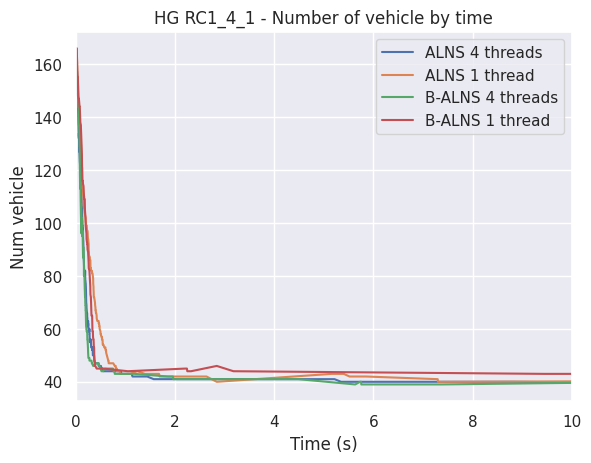
\includegraphics[width=0.9\linewidth]{figures/nv_time_10s_RC1_4_1.png}
    \caption{10s}
    \label{fig:perf_ct_rc1_4_10s}
  \end{subfigure}%
  \begin{subfigure}{.5\textwidth}
    \centering
    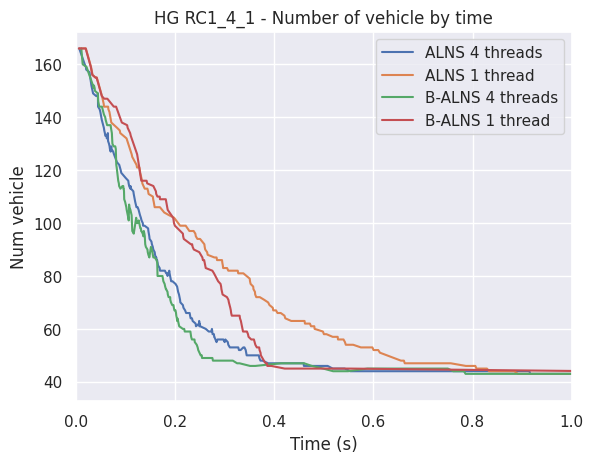
\includegraphics[width=0.9\linewidth]{figures/nv_time_1s_RC1_4_1.png}
    \caption{1s}
    \label{fig:perf_ct_rc1_4_1s}
  \end{subfigure}
  \caption{Số xe sử dụng theo thời gian, cấu hình RC1\_4\_1}
\end{figure}

\subsection{Hiệu quả của thuật toán hủy khác nhau}
Để làm rõ hơn về hiệu quả của thuật toán \textit{hủy tuyến tệ}, ta thí nghiệm với việc chỉ sử dụng riêng lẻ các thuật toán hủy và đo số xe sử dụng theo thời gian. 

\begin{figure}[H] % places figure environment here   
	\centering % Centers Graphic
	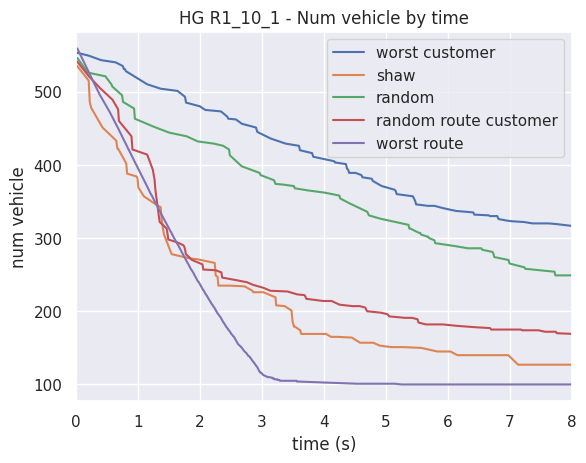
\includegraphics[width=0.7\textwidth]{figures/nv_time_des_10s_R1_10_1.png}
	% \includesvg[scale=1]{figures/core-object}
	\caption{Số xe theo thời gian với các thuật toán hủy khác nhau}
	\label{fig:nv_des_01}
\end{figure}

Hình (\ref{fig:nv_des_01}) biểu diễn số xe sử dụng theo thời gian cho cấu hình \code{R\_10\_1} trong tập dữ liệu Gehring, Hermann, Homberger (1999) \cite{gehring1999parallel}. Thuật toán \textit{hủy tuyến tệ} giúp giảm số xe một cách nhanh chóng trong thời gian đầu chạy ALNS. Điều này cũng khá dễ hiểu do thay vì xóa một số yêu cầu nhất định, thuật toán \textit{hủy tuyến tệ} xóa một tuyến đường hay chính là giảm đi một xe. Ngoài ra thuật toán hủy \textit{Shaw} và thuật toán \textit{hủy ngẫu nhiên với tuyến (random route customer)} cũng cho hiệu quả tốt. Trong quá trình thực nghiệm, chúng tôi nhận thấy rằng, tốc độ thực hiện bước lặp của thuật toán \textit{hủy tuyến tệ} và thuật toán \textit{hủy ngẫu nhiên với tuyến} nhanh hơn đáng kể so với các thuật toán hủy khác. Bản chất hai thuật toán này lựa chọn yêu cầu cần bỏ đi rất nhanh.

Tương tự như hiệu quả về số xe, các thuật toán hủy cũng thể hiện tương tự khi ta biểu diễn giá trị hàm mục tiêu theo thời gian trong hình (\ref{fig:cost_des_01}). Thuật toán \textit{hủy tuyến tệ} tỏ ra rất hiệu quả trong giai đoạn đầu của ALNS. Thuật toán \textit{hủy ngẫu nhiên với tuyến} và thuật toán hủy \textit{Shaw} cũng cho hiệu quả rất tốt không chỉ trong giai đoạn đầu mà còn trong suốt quá trình chạy ALNS (sẽ được chỉ ra trong phần sau).

\begin{figure}[H] % places figure environment here   
	\centering % Centers Graphic
	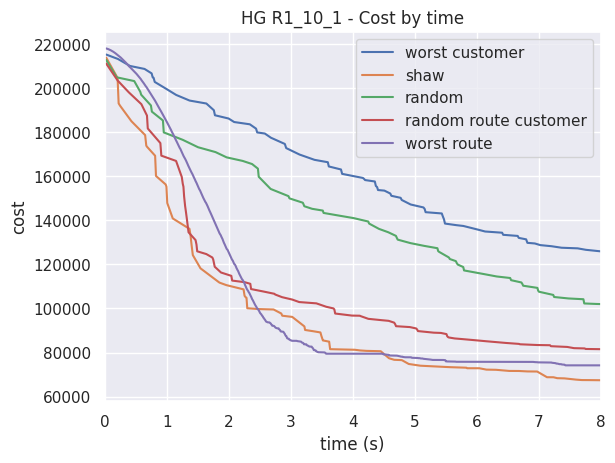
\includegraphics[width=0.7\textwidth]{figures/cost_time_des_10s_R1_10_1.png}
	% \includesvg[scale=1]{figures/core-object}
	\caption{Giá trị hàm mục tiêu theo thời gian với các thuật toán hủy khác nhau}
	\label{fig:cost_des_01}
\end{figure}